\section{Программирование Arduino}
\subsection{Драйвера двигателей}

Для управления шаговыми двигателями используют платы-драйвера, в моем случае это самые распространенные А4988. Их функция заключается в формировании псевдосинусоидальных токов в обмотках шагового двигателя, заставляя его делать шаги или микрошаги. Благодаря подаче сигналов на контакты MS1, MS2, MS3 можно выставить дробление шага от $\frac{1}{2}$ до $\frac{1}{32}$. Дробление шага позволяет увеличить в разы точность позиционирования, путем увеличения количества шагов на оборт, но от этого страдает скорость вращения и момент. В данном проекте, скорость и момент важнее точности, поэтому функция дробления шага не была задействована.

Управление драйвером происходит с помощью трех контактов. Первый, отвечает за включение (enable), без подачи напряжения на этот конакт, драйвер будет игнорировать команды на движение. Наличие сигнала на контакте dir определяет направление последующих шагов. Каждый сигнал на контакте step является командой драйверу сделать шаг двигателем.    

Питание на драйвер приходит в обход платы Arduino, в моем проекте используется 12-ти вольтовый адаптер питания. Если отключить обмотки двигателя, то можно настроить ток драйвера, вращая отверткой потенциометр на плате. Для разных драйверов токи считаются по-своему, в случае с А4988 она выглядит так:

\begin{center}
$I_{raschet} = \frac{I_{nominal\_dvig}}{2.5} = \frac{1.7}{2.5} = 0.68 A $
\end{center}

\begin{figure}[h]
\centering
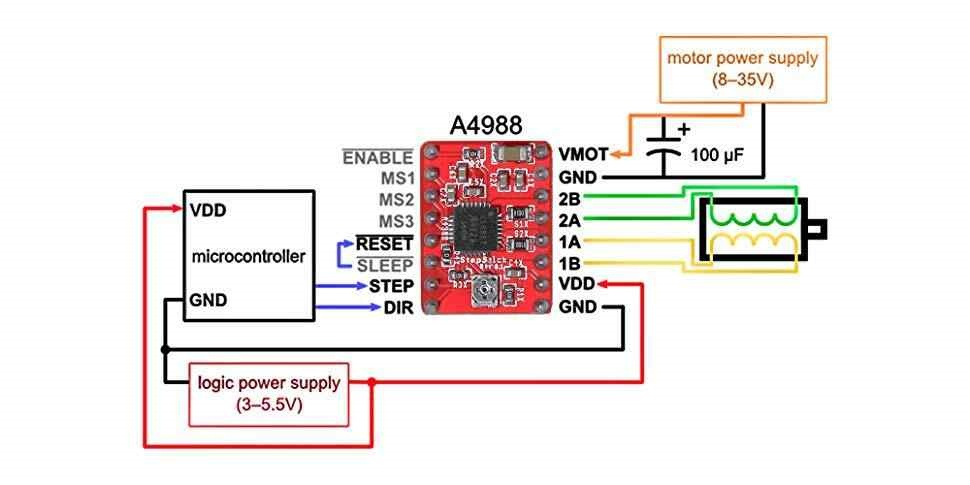
\includegraphics[width=0.8\linewidth]{./image/a4988}
\caption{Схема контактов драйвера шагового двигателя}
\end{figure}

Выставленное значение тока влияет на момент, с которым работает двигатель, на его шумность и силу нагрева. При завышении токов можно увеличить момент, но нагреть двигатель до $90^{\circ}$, что может размягчить пластик, который не держит температуры выше $80^{\circ}$. Занижение токов приведет к понижению шума, вибраций и температуры, но двигатель может начать пропускать шаги из-за недостаточного момента. 

\subsection{Распиновка Arduino CNC Shield}

Arduino CNC Shield продается как готовое решение для самодельных трехосевых станков. Плата создана специально под открытую прошивку GRBL для Arduino. Для взаимодействия с этой прошивкой энтузиасты написали несколько программ для различного использывания CNC станков (фрезеровка, графировка или рисование). Общение с платой происходит с помощью команд gcode, отправляемых по com-порту. Поддерживаются функции плавного набора скорости шаговых двигателей, плавное движение по окружностям и спиралям и другие возможности.

Тем не менее специфика движения дельта-робота заключается в том, что все 3 шаговых двигателя должны работать одновременно. В то время, как в линейных станках одновременно работают только две оси и только в предварительно заложенных функциях, например, по рисованию окружностей. С помощью gcode можно управлять углами поворотов рычагов, через координаты x, y, z. Но нужно понимать, что внутри программы будут одновременно переменные x, y, z, которые обозначают координату в пространстве и x, y, z, которые являются углами.   

\begin{figure}[h]
\centering
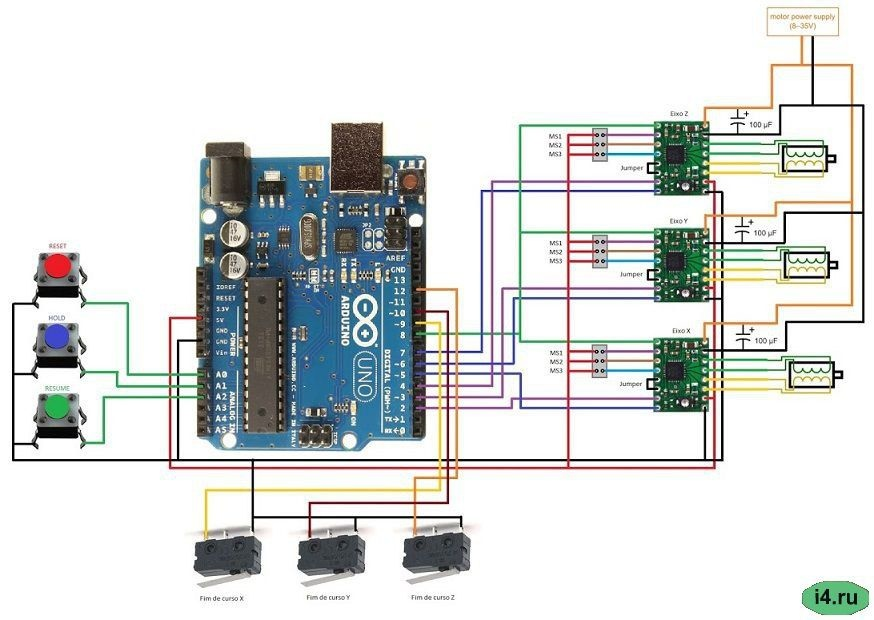
\includegraphics[width=0.8\linewidth]{./image/shield}
\caption{Схема распиновки Arduino CNC Shield}
\end{figure}

В качестве тренировки и для набора практического навыка, решил самостоятельно написать скетч. Первым делом необходимо объявить рабочие пины Arduino:

\begin{lstlisting}[style=uno,caption=Объявление пинов Arduino]
int step1 = 2;
int step2 = 3;
int step3 = 4;

int dir1 = 5;
int dir2 = 6;
int dir3 = 7;

int pwr = 8;

int kon1 = 9;
int kon2 = 10;
int kon3 = 11;

void setup() {
  Serial.begin(115200);
  pinMode(step1, OUTPUT);
  pinMode(step2, OUTPUT);
  pinMode(step3, OUTPUT);
  pinMode(dir1, OUTPUT);
  pinMode(dir2, OUTPUT);
  pinMode(dir3, OUTPUT);
  pinMode(pwr, OUTPUT);
  pinMode(kon1, INPUT);
  pinMode(kon2, INPUT);
  pinMode(kon3, INPUT);
  }

\end{lstlisting}

Я создаю переменные, обозначающие номер порта, чтобы иметь возможность в случае необходимости менять порт, не переписывая код скетча целиком. Порты с 2 по 8 назначаю выходами и с помощью них буду отправлять управляющие сигналы на драйвера. Порты с 9 по 11 назначаются входами, в случае если в процессе выполнения движения рычаг нажмет на концевик, то на один из этих портов придет сигнал. К сожалению, оба концевика: минимальное положение и максимальное положение, у данной паты выведены на 1 пин. Поэтому определить, какой именно концевик сработал можно только по направлению движения двигателя.  


\subsection{Основная функция}

Под основной функцией в скетче подразумевается управление Arduino с помощью команд, принимаемых через com-порт. Так как ком порт ограничен тем, что мы можем отправлять только восьмибитные сообщения, представляющие собой число от 0 до 256, конвертируемое в символ ASCI кодировки, то и команды представляют собой 1 символ. Для передачи числа в формате Int, представляющее собой 4 байта, необходимо со строны компьютера разбить перменную Int на массив из 4 символов float, и передовать их по очереди. Со стороны Arduino существует функция Serial.parseInt, которая собирает 4 символа float, обратно в переменную типа Int. На данный момент, я ограничился двумя командами: возврат каретки в исходную позицию и перемещение каретки в новую координату. Начальная позиция в даннном случае это углы $\theta_{i}$ равные $-15^{\circ}$. Углы необходимо перевести в шаги двигателей и работать с ними.
\begin{center}
    $n_{shagov} = \frac{\theta_{max} - \theta_{min} }{360^{\circ}}* N_{dvig} * K_{reductor} = \frac{90^{\circ}+15^{\circ}}{360^{\circ}}*200*6 = 350$
\end{center}

Количество шагов от минимального до максимального положения является отношением полного угла к полной окружности, домноженное на количество шагов на оборот шагового двигателя и на коэффицент передачи редуктора. Получается, что для прохождения рычага до крайнего положения необходимо сделать 350 шагов, что больше 256, поэтому мы не можем использовать 8 битные числа для передачи изменения координаты, а вынуждены использовать переменные типа Int.

Для того, чтобы узнать на какие углы необходимо переместить рычаги необходимо дважды решить решить обратную задачу управления. Первый раз мы рассчитываем углы $\theta_{i}$ для настоящего положения в пространстве, а второй раз для последующего положения. И только вычитая результат первого решения из второго, мы получим значение изменения углов. 
В скетче ардуино, я завожу 9 переменных, отвечающих за хранение состояния углов: текущие значение $\theta_{i}$, новые значения, полученные по com-порту, и $\Delta_{i}$, разница между ними. 

Плата Arduino в бесконечном цикле ожидает сигнала по com-порту. Если будет получена буква H, что обозначает home, то будет вызвана функция move\_home(). Важно, что именно перед вызовом функции движения, я отключаю порт pwr, тем самым разрешая работу драйверам. После выполнения функции двиения, возвращаем драйверам запрет на движение и посылаем в com-порт букву Y, подтверждение для компьютера, что функция выполнена адекватно

Если получена буква С, что обозначает change position, Arduino по очереди запрашивает значение координат, в которые необходимо перенести каретку. Происходит расчет $\Delta_{i}$, снимается запрет на работу драйверов и выполняется функция движения каретки.

Подсчет текущего значения углов $\theta_{i}$ будет происходить внутри функций движения.
\begin{lstlisting}[style=uno,caption=Основная функция скетча]
void loop() {
    if (Serial.available() > 0) {

        val = Serial.read();
        Serial.write(val);

        if (val == 'H') { 
            digitalWrite(pwr,LOW);
            move_home();
            digitalWrite(pwr,HIGH);
            Serial.print('Y');}

        if (val == 'C') {
            Serial.print('X');
            NEW_teta1 = Serial.parseInt();
            Serial.print('Y');
            NEW_teta2 = Serial.parseInt();
            Serial.print('Z');
            NEW_teta3 = Serial.parseInt();
            
            delta1 = NEW_teta1 - teta1;
            delta2 = NEW_teta2 - teta2;
            delta3 = NEW_teta3 - teta3;
            
            digitalWrite(pwr,LOW);
            change_location();
            digitalWrite(pwr,HIGH);

            Serial.print('Y'); 

            }
    }
}
\end{lstlisting}

\subsection{Функция возврата каретки домой}

Функция возврата каретки домой устроена по принципу, движения двигателя до тех пор, пока не появится сигнал на соответсвующем порту, к котрому подключен концевик. Цикл while выполняется до тех пор пока все концевики не будут активированы. В условии использованно логическое ИЛИ и утверждение, что концевики в неактивированном состоянии. Пока хоть один из них будет неактивирован, цикл будет выполняться. Внутри цикла происходит дополнительная проверка на концевики для каждого двигателя, перед выполнением функции движения. Это делается потому, что скорее всего рычаги придут в крайние положения не синхронно.

После выполнения цикла, все рычаги должны оказаться в начальной позиции, соответсвенно можно обнулить глобальные переменные текущих значений $\theta_{i}$.

\begin{lstlisting}[style=uno,caption=Функция возврата каретки домой]
int move_home(){
    while(digitalRead(kon1)==LOW|| //неправильный перенос строки
            digitalRead(kon2)==LOW||
                digitalRead(kon3)==LOW){
        if(digitalRead(kon1)==LOW){move_teta1(-1);}
        if(digitalRead(kon2)==LOW){move_teta2(-1);}
        if(digitalRead(kon3)==LOW){move_teta3(-1);}
        }
    teta1 = 0;
    teta2 = 0;
    teta3 = 0;
}
\end{lstlisting}

Функции изменения угла рычага однотипны, создают два сигнала на нужные выходы, с некоторой задержкой. В зависимости от необходимого направления движения, задается положительное или отрицательное k. В зависимости от знака, на пин dir либо подается, либо не подается напряжение. После подачи сигнала на направление, необходимо дать задержку, в данном случае это t миллисекунд. После подачи сигнала step, делается вторая задержка для совершения шага. Величины задержек зависят от скорости срабатывания платы микроконтроллера. Для драйвера A4988 задержки очень большие, двигатель не может начать движение, если задать их меньше 500 микросекунд. Это связано с резким спадом момента на роторе, так как управляющий ток не успевает нарастать за такой промежуток времени. Если уменьшать задержки уже вращающегося двигателя, то можно плавно опустить их до 250 микросекунд, но при любом толчке происходит пропуск шагов и двигатель останавливается. Так как мне важна стабильная работа двигателей, без пропуска шагов и с хорошим моментом, я решил использовать задерки в 1 миллисекунду. В своем предыдущем проекте, когда использовал трехканальный драйвер SMD-303 совсем другой ценовой категории, то использовал задержки в 50-60 микросекунд. Этот опыт оказался вредным, так как выставляя низкие задержки, я потратил много времени, считая что двигатели не могут повернуть редуктор, так как клинит шестерни. Я повышал задержки до 200 микросекунд, но это не давало результата, я пересобирал конструкцию, печатал новые шестеренки и тратил время и силы впустую.   

\begin{lstlisting}[style=uno,caption=Функция управляющяя шаговым двигателем]
int move_teta1(int k){
    if (k>0) {
    digitalWrite(dir1,HIGH);
    delay(t);
    digitalWrite(step1,HIGH);
    delay(t);
    teta1++; }
    if (k<0) {
    digitalWrite(dir1,LOW);
    delay(t);
    digitalWrite(step1,HIGH);
    delay(t);
    teta1--; }
}
\end{lstlisting}

\subsection{Функция изменения координаты}

Логика данной функции заключается в поочередном совершении шагов двигателями до тех пор, пока разница в координатах $\Delta_{i}$ не станет равной нулю. Цикл while выполняется тогда, когда есть отличная от нуля разница в координатах. Используется логическое ИЛИ. Внутри цикла происходит повторная проверка, что разница не равно нулю и одновременно не задействованны концевики. После этого, в зависимости от знака разницы, вызывается функция движения в определенную сторону, а разница уменьшается по модулю на единицу. Если разница по одной из координат станет равной нулю раньше остальных или будет задействован концевик, этот двигатель прекратит движение и будет ждать остальных. В случае, если рычаг активировал концевик до того, как разница стала нулевой, то на этот случай происходит обнуление разницы, чтобы цикл не превращался в бесконечный.

\begin{lstlisting}[style=uno,caption=Функция изменения координаты]
int change_location(){
    while(delta1 != 0||delta2 != 0||delta3 != 0){
        if( delta1 !=0 && digitalRead(kon1)==LOW) {
            if( delta1 > 0 ) {move_teta1(1); delta1--;}
            else {move_teta1(-1); delta1++;}}
        else{delta1 = 0;}
        if( delta2 !=0 && digitalRead(kon2)==LOW) {
            if( delta2 > 0 ) {move_teta2(1); delta2--;}
            else {move_teta2(-1); delta2++;}}
        else{delta2 = 0;}
        if( delta3 !=0 && digitalRead(kon3)==LOW) {
            if( delta3 > 0 ) {move_teta3(1); delta3--;}
            else {move_teta3(-1); delta3++;}}
        else{delta3 = 0;}
    }
}
\end{lstlisting}

Слабое место данной функции в том, что двигатели поочередно делают шаги. Один шаг занимает 2 миллисекунды, а это значит, что пока один двигатель двигается, два других будут проставивать в течение 4 миллисекунд. Эксперементируя с данным скетчем, в какой-то момент я придумал, каким образом надо изменить функцию, чтобы двигатели двигались действительно одновременно. Изначально, мне не удавалось победить то обстоятельство, что у каретки есть шесть степеней свободы, что подразумевает необходимость написания шести разных функций, но решение нашлось.

В новой функции нет вызова других функции управления двигателями, так как это оказалось ненужным. Цикл while как и в прошлый раз выполняется до тех пор, пока хоть одна из переменных $Delts_{i}$ отлична от нуля. Внутри цикл делится на две половины. В первой половине, в зависимости от знака разницы посылаются сигналы dir, отвечающие за направление движения. Если разница равна нулю, сигнал будет послан, но к ошибке это не приведет. После этой операции происходит необходимая задержка. Во второй половине цикла происходит проверка на отличие разницы от нуля и срабатывание концевика. Если разница отлична от нуля и концевик не сработал, то можно отправлять сигнал на шаг. После чего остается только изменить глобальное значение угла и разницы на единицу. Если сработал концевик, но разница при этом не равна нулю, она приравнивается к нулю, чтобы цикл while не становился бесконечным.  

Таким образом мне удалось реализовать одновременное функционирование двигателей, в независимости от направления движения и разнице количества шагов. Более того, так как двигатели работают одновременно и имеют общую задержку, ее можно очень просто менять во времени, тем самым разгоняя двигатели. В моем случае, драйвера очень плохо реагируют на разгон, поэтому я меняю задержку с 1000 микросекунд до 500 микросекунд в течение 22 шагов, по квадратичному закону. Возможно, дальнейшие эксперименты позволят выжать из драйверов большие показатели, возможно стоит завысить токи, но это требует дальнейших испытаний. И важно придумать способ отлавливать пропущенные шаги, так как двигатель иногда может пропускать шаги без остановок, но отследить это без обратной связи невозможно.

\begin{lstlisting}[style=uno,caption=Усложненная функция с плавным разгоном]
int hard_change_location(){
    int k = 0;
    while(delta1 != 0||delta2 != 0||delta3 != 0){

        if(del2ta1 > 0) {digitalWrite(dir1,HIGH);}
            else {digitalWrite(dir1,LOW);}
        if(delta2 > 0) {digitalWrite(dir2,HIGH);}
            else {digitalWrite(dir2,LOW);}
        if(delta3 > 0) {digitalWrite(dir3,HIGH);}
            else {digitalWrite(dir3,LOW);}

        delayMicroseconds(1000 - k*k);

        if(delta1 !=0 && digitalRead(kon1)==LOW) {
            digitalWrite(step1,HIGH);
            if(delta1 > 0) {delta1--; teta1++;}
                else{delta1++; teta1--;}}
        else {delta1=0;}

        if(delta2 !=0 && digitalRead(kon2)==LOW) {
            digitalWrite(step2,HIGH);
            if(delta2 > 0) {delta2--; teta2++;}
                else{delta2++; teta2--;}}
        else {delta2=0;}

        if(delta3 !=0 && digitalRead(kon3)==LOW) {
            digitalWrite(step3,HIGH);
            if(delta3 > 0) {delta3--; teta3++;}
                else{delta3++; teta3--;}}
        else {delta3=0;}

        delayMicroseconds(1000 - k*k);

        if (k < 22) {k++;}
    }
}
\end{lstlisting}

\subsection{Вывод}

Данным скетчем реализован минимальный функционал, необходимый для управления роботом. Arduino умеет возвращать каретку в начальное положение, отсчитывать координаты, и перемещаться на заданные через com-порт величины углов. Важно, что благодаря реализованной фунции, двигатели совершают шаги единовременно, без простоя. Есть пространство для улучшения механизма разгона двигателей, возможно, получится реализовать дополнительно торможение по квадратичному закону.Ощущается упор в возможности драйвера a4988, возможно стоит расмотреть другие варианты драйверов.  

